\chapter{躯体治疗}

\section{概  述}

精神障碍的躯体治疗主要包括药物治疗、物理治疗和功能外科手术治疗。药物治疗是临床最常用的治疗方法;物理治疗目前主要是电抽搐治疗,用于严重抑郁、木僵和兴奋躁动的控制;功能外科手术治疗用于一些难治性精神障碍的治疗,同时符合功能外科手术治疗的适应证。

\section{药物治疗}

精神药物(psychotropic
drugs)是指主要作用于中枢神经系统以影响精神活动的药物。这类药物在治疗剂量内并不影响意识和智能。

Cade
1949年最早提出锂盐可以治疗躁狂,但因当时未能解决其毒性反应,故未引起广泛重视。1950年法国化学家Paul
Charpentier合成了一种新的酚噻嗪类衍生物氯丙嗪,当时主要用于辅助麻醉。1952年5月Jean
Dely和Pierre
Deniker首先报道,应用氯丙嗪治疗精神病人获得成功,从此翻开了精神疾病治疗学新的一页,首次点燃了人类用药物治疗疾病的希望,使精神病学有了炫目的现代医学的色彩。

随着精神药物品种的增多,就有了分类的必要,一般分为四类:

1.抗精神病药(anti-psychotics) 主要用于治疗精神分裂症,对幻觉、妄想及行为紊乱等精神病性症状疗效较佳。

2.抗抑郁药(anti-depressants) 主要用于治疗各种抑郁。

3.抗焦虑药(anti-anxiety
drugs) 主要用于治疗焦虑症状,也可作为催眠药用。

4.抗躁狂药(anti-manic
drugs)和情感稳定剂(mood-stabilizers) 主要用于躁狂和双相情感障碍。

\section{抗精神病药}

抗精神病药(anti-psychotics)是一组主要用于治疗精神分裂症及其他精神病性精神障碍的药物。曾被赋予许多不同的术语,如精神松弛剂(psycholeptics)、安适剂(ataraxics)、强安定剂(major
tranquillisers)、神经阻滞剂(neuroleptics)等,这些名词目前已被废弃,作为简单描述性术语------抗精神病药,正逐步被广泛接受。

\subsection{分类}

其分类见表\ref{tab18-1}。

\begin{table}[ht]
    \caption{抗精神病药}
    \label{tab18-1}
    \centering
    \begin{tabular}{llll}
    \toprule
    & & 二甲胺类&氯丙嗪\\
    \midrule
    \multirow[t]{6}{3cm}{第一代抗精神病药(传统抗精神病药、典型抗精神病药) }&  酚噻嗪&哌嗪类&奋乃静、氟奋乃静、三氟拉嗪
\\
~&&哌啶类&甲硫哒嗪、哌普嗪
\\
~&硫杂蒽类 && 泰尔登、三氟噻登、氯噻登\\
~&丁酰苯类&&氟哌啶醇、五氟利多、哌迷清\\
~&萝芙木类&&利血平\\
~&苯酰胺类&&舒必利\\
\multirow[t]{3}{3cm}{第二代抗精神病药(新型抗精神病药、非典型抗精神病药)}&5-羟色胺/多巴胺受体平衡拮抗剂&&
维思通、齐哌西酮\\
~&多巴胺受体作用&&
奥兰扎平、奎太平、氯氮平\\
~&多巴胺系统稳定剂&&
阿立哌唑\\
    \bottomrule
    \end{tabular}
\end{table}

\subsection{第一代抗精神病药物}

第一代抗精神病药物亦被称为传统抗精神病药或经典抗精神病药,以氯丙嗪、氟哌啶醇等为代表。其共同特点有:主要阻断中枢多巴胺受体,对阳性症状有效,对阴性症状、认知损害基本无效,锥体外系反应严重,引起血浆催乳素增高。

\subsubsection{化学结构}

酚噻嗪类的基本结构如下:
\begin{center}
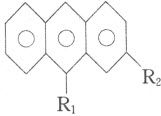
\includegraphics[width=.3\textwidth]{./images/Image00015.jpg}
\end{center}
R\textsubscript{1}
位上基团决定药物的效价,一般规律为F\textgreater{}Cl\textgreater{}H;R\textsubscript{2}
基团的不同,决定酚噻嗪类亚型的划分。化学结构中含氯者,对心脏、肝功能、血象影响较大,含氟者,具有振奋激活作用,适用于淡漠、退缩的病人。有人按抗精神病药效价简单分为强效和低效两大类,强效抗精神病药有效剂量低,镇静作用弱,较少自主神经功能副作用,对心脏、肝脏、血象影响小,但锥体外系副作用较重。代表性药物有三氟拉嗪、氟哌啶醇、五氟利多等。低效抗精神病药,治疗剂量高,有较强的镇静作用和自主神经系统反应,对心脏、肝脏、血象影响较大,锥体外系反应轻。代表性的药物有氯丙嗪、泰尔登、甲硫哒嗪、氯氮平等。

\subsubsection{药理作用}

1.对中枢神经系统的影响

(1)镇静作用:引起感觉阈的轻度增高,兴奋性降低,不引起皮层明显抑制,遇到刺激仍有完善的觉醒反应,其镇静机制是阻断脑干网状结构上行激活系统外侧部的α受体。

(2)抑制条件反射:能使凶猛的动物驯服,不能抑制非条件反射。

(3)镇吐作用:小剂量氯丙嗪能抑制延脑第四脑室底部极后区催吐化学感受器,大剂量直接抑制呕吐中枢。小剂量氯丙嗪即可对抗去水吗啡(兴奋延脑第四脑室极后区催吐化学感受器)引起的呕吐,不能对抗硫酸铜的催吐作用,硫酸铜的催吐作用是由于刺激胃黏膜,反射性引起呕吐中枢兴奋所致,大剂量氯丙嗪才能对抗。

(4)降温作用:抑制下丘脑体温调节中枢,使体温调节功能减低,导致体温随外界温度而变化。人工冬眠与物理降温同时应用,降温作用明显。但在炎热天气,则可使体温升高,导致中暑。

(5)对脑电的影响:引起脑电频率的改变,出现大量θ波,δ波稍增多,β波减少,可出现爆发活动及峰形波,同步增加伴电压增高。有人观察抗精神病药治疗精神分裂症无效时,脑电图一般无变化,极快波减少越多,疗效越佳。出现异常大幅波,预示病人对药物不能耐受。

(6)精神病作用:中枢神经系统目前已知存在四条多巴胺神经通路,黑质-纹状体、结节-漏斗、中脑-边缘系统、中脑-大脑皮层,氯丙嗪抗精神病的作用机制可能是阻断中脑-边缘系统、中脑-大脑皮层通路的多巴胺受体有关。

2.对自主神经系统的影响

(1)降压作用:氯丙嗪可阻断血管上α受体,扩张血管,降低血压,故可导致体位性低血压。血压下降可反射性地引起心动过速。降压作用由于连续用药而产生耐受,不适合高血压的治疗。当氯丙嗪过量引起血压下降时,不能用肾上腺素纠正。这是因为血管上同时存在α、β受体,α受体兴奋,血管收缩,血压升高;β受体兴奋,血管扩张,血压下降。肾上腺素既能兴奋α受体,又能兴奋β受体,在正常情况下表现出α受体兴奋的作用。当氯丙嗪过量中毒时,阻断了血管上α受体,使得肾上腺素不能与α受体结合,只能作用于β受体,导致血管进一步扩张,血压进一步下降。因此氯丙嗪过量引起的血压下降不能用肾上腺素纠正,只能用仅兴奋α受体对β受体无作用的去甲肾上腺素或阿拉明。

(2)缩瞳作用:氯丙嗪阻断虹膜辐射肌上的α受体,辐射肌松弛,瞳孔缩小。

(3)抗胆碱能作用:氯丙嗪具有微弱的抗胆碱能作用,可引起口干、便秘、视物模糊等。

3.对内分泌的影响 结节-漏斗通路中的多巴胺可促使下丘脑分泌多种激素,从而间接促进多种激素的分泌。氯丙嗪阻断该通路的多巴胺受体,减少下丘脑释放催乳素抑制因子,从而引起持续性催乳素增高,乳房肿大及泌乳,抑制促性腺激素的释放而使排卵延迟、月经紊乱,抑制ACTH的释放而使糖皮质激素分泌减少。

\subsubsection{药代动力学}

氯丙嗪口服、肌注均易吸收,约有90%与血浆蛋白结合,口服后2~4小时血药浓度达高峰,能够分布到脑、肺、肝、肾等器官,脑内浓度是血浆浓度的4~5倍。半衰期的个体差异较大,为8~35小时,体内可以积蓄,主要在肝脏中代谢,代谢产物复杂。

\subsubsection{临床应用}

1.治疗精神分裂症和其他精神病性障碍,不应滥用于神经症或作催眠药应用。

2.人工冬眠用于创伤性休克、中毒性休克、高烧、甲亢危象的辅助治疗,增加肌体对有害刺激的耐受力。

3.用于多种药物和疾病引起的呕吐,如洋地黄、吗啡、尿毒症及癌症引起的呕吐,也可用于顽固性呃逆。

\subsubsection{副反应}

1.精神方面

(1)过度镇静:病人表现无力、嗜睡。

(2)药源性精神病:①精神运动性兴奋:在治疗过程中出现明显的兴奋躁动或使原有精神运动性兴奋加剧,表现为焦虑不安、激动、凶狠、敌意、冲动、攻击行为。以强效药物或有轻度脑器质性损害者较易出现。②意识障碍:有1%~3%病人出现不同程度的意识障碍。多见于用药早期,午后晚间明显;大剂量用药或剧增骤停,联合用药,特别是与三环类抗抑郁药或抗胆碱能药物联用,老年人或有器质性病变者易出现。③药源性抑郁:病人表现为焦虑、烦躁、消极悲观、情绪不稳、自责自罪、自残自伤等,以利血平、氟哌啶醇、氯丙嗪、奋乃静、三氟拉嗪较易发生。④紧张症候群:主要表现缄默、木僵、违拗、蜡样屈曲,重者吞咽困难,生活不能自理。

2.神经系统方面

(1)惊厥:可诱发癫痫
,以低效价药物为多。

(2)锥体外系反应:锥体外系反应的发生率与药物的种类、剂量、疗程及个体因素有关,发生时间最早可在服药后0.5~48小时出现,多数在用药后2~5周内发生。①药源性类帕金森综合征:表现为肌肉强劲、震颤、运动不能、自主神经功能紊乱。②静坐不能:表现不可控制的烦躁不安、不能安定、反复走动或原地踏步。③急性肌张力障碍:表现个别肌群持续痉挛,表现为各种奇怪动作或姿势,如下颌不能闭合,面肌、颈肌痉挛、口眼歪斜、角弓反张、扭转性痉挛。静坐不能多见于中年女性,急性肌张力障碍多见于男性青少年。处理:减药、停药或使用拮抗剂。产生的机制是氯丙嗪阻断了黑质-纹状体通路的多巴胺受体,使得纹状体中多巴胺功能减弱,乙酰胆碱功能增强而引起。④迟发性运动障碍:多发生于长期大剂量用药的病人,发生率为5%~20%,老年、女性、伴脑器质性疾病者发生率较高。临床表现为不自主的、有节律的刻板式运动,其特点为肌张力低下。这些症状在睡眠时消失,情绪紧张、激动时加重,可以与药源性帕金森综合征同时存在,且症状往往被掩盖,在减药或停药后迅速暴露。处理:减药、停药或换用锥体外系反应小的药物,停用一切抗胆碱药物,对症处理,给予非那根、安定、神经营养剂等。目前认为发病机制是由于多巴胺受体去神经增敏所致。

3.自主神经系统副作用

(1)抗胆碱能作用:表现为口干、视物模糊、心动过速、便秘、肠麻痹、尿潴留、眼压升高等。

(2)抗肾上腺素能作用:头昏、头晕、体位性低血压等。

(3)抑制体温调节中枢:在炎热夏季、皮肤散热功能降低,可导致高热、中暑。

(4)性功能障碍:偶可引起勃起困难、射精不能、性欲减退。

(5)心电图改变:常见T波改变、ST段压低、QRS波增宽、QT延长、心律改变或传导阻滞。

4.内分泌方面的影响 女性病人排卵延迟、月经周期紊乱、溢乳、性欲改变,常可出现体重增加。

5.肝脏副作用 20%~30%的病人在服药1个月内有一过性谷丙转氨酶升高,少数病人出现肝细胞内微胆管阻塞性黄疸,多数在用药后2~4周内发生,目前认为这是一种过敏反应。

6.血液系统副作用 氯丙嗪对骨髓有毒性作用,抑制骨髓造血功能,导致粒细胞减少或再生障碍性贫血。

7.皮肤方面副作用 可出现药疹、接触性皮炎、光敏性皮炎、皮肤色素沉着。

8.恶性综合征 这是一种少见而危险的副反应,表现为持续高热,锥体外系症状加剧,全身肌张力增高,自主神经功能紊乱,碱性磷酸酶增高。

\subsubsection{给药方法}

1.剂量 以达到理想治疗效果的最低有效量和最小的副作用为标准,不应千篇一律,力求剂量个别化。有时中小剂量病人病情无进步,大剂量有明显进步;有时则相反,中小剂量反应好,大剂量病情反而恶化。常用剂量范围为300~600mg/d。

2.显效时间 恰当的剂量兴奋躁动在一周左右控制,幻觉妄想需要1~2个月,若仍不见效,可能剂量不足或对此药不敏感。恰当的剂量必然会出现疗效或锥体外系反应,若两者均不出现,可能是剂量不足。

\subsubsection{硫杂蒽类}

以泰尔登为代表,抗兴奋躁动、幻觉妄想作用不如氯丙嗪,镇静作用较强,具有较弱的抗抑郁、焦虑作用,适用于带有焦虑抑郁情绪的精神分裂症,其抗肾上腺素和抗胆碱能作用较弱,锥体外系反应也较轻,易引起癫痫
发作,常用剂量为100~600mg/d,另外还有三氟噻登、氯噻登。

\subsubsection{丁酰苯类}

以氟哌啶醇为代表,主要用于控制兴奋躁动、躁狂状态、幻觉妄想为主的精神障碍,对慢性精神分裂症有一定的振奋激活作用,对儿童行为障碍如活动过度、多发性抽动秽语综合征疗效较佳。抗肾上腺素与抗胆碱能作用弱,阻断多巴胺作用强,镇静作用弱,镇吐作用强。副作用为锥体外系反应重,对肝肾功能、血象、心血管影响小,少数可导致失眠、药源性抑郁,常用剂量为8~40mg/d。另外还有哒哌啶醇、五氟利多等。

\subsection{第二代抗精神病药}

亦被称为新型抗精神病药或非典型抗精神病药,以氯氮平为代表,其共同特点为,对中枢多种受体有亲和力,锥体外系副反应小或无,作用广泛,对阳性、阴性和认知缺陷症状均有效,基本不影响催乳素水平或影响很小。

\subsubsection{氯氮平}

氯氮平于1959年合成,化学结构与丙咪嗪相似,最初作为抗抑郁药使用,不久发现具有抗精神病作用,而基本无抗抑郁作用,很快就得到广泛应用。由于1974年芬兰出现8例因使用此药导致粒细胞缺乏,且部分病人死亡,之后又有陆续报道,此药的应用明显减少。美国Kane
1988年发现此药对难治性病人有效,才开始此药的新纪元。氯氮平被认为可能是目前最有效的抗精神病药,且只要常规监测白细胞,此药具有较好的安全性。氯氮平与第一代抗精神病药区别在于其与D\textsubscript{2}
受体的亲和力很低,可与其他广泛的不同类型受体结合,在多巴胺系统中,可与D\textsubscript{1}
、D\textsubscript{2} 、D\textsubscript{3} 、D\textsubscript{4}
受体结合,且与D\textsubscript{4}
亲和力较高;与5-羟色胺受体也有较高的亲和力,特别是5-HT\textsubscript{2A}
、5-HT\textsubscript{2C} 、5-HT\textsubscript{6} 、5-HT\textsubscript{7}
,另外还与α\textsubscript{1} 和α\textsubscript{2} 、H\textsubscript{1}
、M受体结合。

氯氮平控制精神运动性兴奋奏效快,控制幻觉妄想与氯丙嗪相似,对慢性退缩症人也有一定疗效,对经典抗精神病药物治疗无效的病人,改用氯氮平治疗大约有1/3的病人仍可获得显效。常见副作用有流涎、便秘、低血压、心动过速、心电图改变、诱发癫痫
,偶可引起粒细胞减少或缺乏,无锥体外系反应。常用剂量为200~600mg/d。

\subsubsection{奥兰杂平(奥氮平)}

奥氮平是一种噻吩苯二氮䓬
类衍生物,其结构和药理特性与氯氮平相似,与多种神经递质受体有亲和力。口服后5小时达峰浓度,健康年轻人清除半衰期为27~38.6小时,主要经肝脏代谢,其代谢产物无活性。主要不良反应为过度镇静、口干、便秘、肝脏转氨酶增高和体重增加。常用剂量为5~15mg/d。

\subsubsection{利培酮(维思通)}

维思通对中枢多巴胺D\textsubscript{2} 受体和5-HT\textsubscript{2}
受体均有较强的拮抗作用,有人认为维思通拮抗边缘系统多巴胺受体,缓解阳性症状;拮抗5-羟色胺受体,缓解阴性症状;对黑质纹状体通路中5-羟色胺受体的拮抗,可促进多巴胺的释放,降低锥体外系的副作用。口服易吸收,服药后1小时达峰浓度,主要在肝脏中代谢,其代谢产物9-羟利培酮仍具活性,快代谢型者消除半衰期利培酮为3小时,9-羟利培酮为20小时,慢代谢型者消除半衰期利培酮为20小时,9-羟利培酮为20~29小时。主要不良反应为锥体外系反应,与剂量有明显的相关性,超过6mg/d,锥体外系发生率显著增加,低于6mg/d,锥体外系发生率明显减少。该药无明显的镇静作用。常用剂量为2~6mg/d。

\subsubsection{喹硫平}

喹硫平是一种二苯硫西平类药物,与5-羟色胺受体的亲和力远高于多巴胺α\textsubscript{2}
受体亲和力,与组胺受体和α肾上腺素能受体也有较高的亲和力,与胆碱受体几乎没有亲和力。口服迅速吸收,在1~1.5小时后达峰浓度,主要由细胞色素P450
3A4系统在肝脏代谢,代谢产物无活性。喹硫平总体耐受性较好,0.5%病人出现心电图QTc间期延长。常用剂量150~750mg/d。

\subsubsection{阿立哌唑}

阿立哌唑是一种喹诺酮衍生物,为多巴胺部分激动剂和部分激动5-HT\textsubscript{1A}
和拮抗5-HT\textsubscript{2A}
受体的作用,因此被称为多巴胺-5-羟色胺系统稳定剂。吸收良好,生物利用度为87%。总体耐受性较好,少部分病人有锥体外系反应,其主要表现为静坐不能。常用剂量为10~30mg/d。

\subsection{用药原则}

1.个体化原则 每个病人对精神药物的耐受性、疗效,存在明显的个体差异,药物的选择和剂量要个体化,不能千篇一律,参考病人的年龄、性别、躯体情况,是否初次治疗等因素来决定药物的剂量。

2.剂量原则 最小剂量达到最佳疗效。剂量过低达不到疗效,剂量过大有时不但不能进一步提高疗效,反而导致许多副作用。恰当的剂量治疗一段时间,必然会出现疗效或副作用,如两种效应都不出现,要高度怀疑病人未服或少服药,其次考虑剂量不足。

3.药物选择 ①根据靶症状:各种精神药物均有各自的靶症状,依据病人的症状选择药物。②病人既往用药经验:如果过去同样症状用某药有效,这次仍可能有效;同样上次无效,这次仍可能无效。但也有例外。③借鉴家族史:如家族中有同样的患者对某药有效,则可能对此病人也有效。

4.疗程 一般从达到治疗剂量之日开始计算,急性病人观察4~6周,病情无效可考虑换药。慢性病人要延长观察时间,有人认为需2~3个月,甚至半年,无效方可考虑换药。

\subsection{联合用药}

支持此观点的理由:①单一用药疗效,同类药物联用疗效可能相加,副作用因各种药物的剂量不大而可能减少;②各种精神药物作用的靶症状不相同,合用可兼顾、全面;③各种精神药物的作用机制不尽相同,疗效可互补。反对此观点的理由:①合并用药并没有减少剂量,相反按效价折算,总量大为超过单一用药的有效剂量,而每种药物因合并用药而剂量不足,反而达不到治疗量,结果疗效没有增加,副作用却增加;②按照突触药理学的观点,药物联用是协同或拮抗作用,难以确定;因而疗效的增加或减弱也难以确定,但副作用增加;③临床研究亦证明联合用药不能提高疗效,但副作用增加。

目前国内的观点:尽可能地单一用药,不主张联合用药,只有当单一用药无效时方可考虑联合用药,且不超过两个。

1.抗精神病药与抗抑郁药的联用 对伴有抑郁症状的精神分裂症,采取合用可收到较好的效果,对分裂情感性精神病和带有精神病性症状的抑郁症亦可。但对精神分裂症无抑郁症状的病人没有单用抗精神病药治疗效果好,相反还可能恶化精神分裂症症状。对无精神病性症状的抑郁症,联用没有单用抗抑郁药治疗效果好。有人报道新型抗精神病药联用SSRIs治疗慢性精神分裂症比单一用药效果好。

2.抗精神病药与锂盐的联用 锂盐虽为躁狂治疗的首选药物,但由于起效时间慢,若与抗精神病药联用可较快地控制症状。Cohen报道54例锂盐合并氟哌啶醇治疗的病人,有4例出现不可逆的脑损害,这一情况是由于血清锂浓度过高,长期合用所致。目前认为两者短期合用是有益的。

3.抗精神病药物与镇静催眠药的联用 抗精神病药可加强麻醉药、催眠药等的作用,联用时注意过度镇静。氯丙嗪与巴比妥类药联用时,巴比妥类药可诱导肝细胞微粒体酶的活性,加速氯丙嗪的代谢。

4.抗精神病药物与抗震颤药的联用 目前国内的观点为,除非出现锥体外系症状,尽可能不用或少用抗震颤药,不能作为抗精神病药锥体外系反应的常规、预防用药。理由是:①不是所有的病人均出现锥体外系反应,约有61.1%的病人并不出现锥体外系症状;②抗震颤药物本身有副作用;③增加迟发性运动障碍的发生率;④降低氯丙嗪的血浓度,从而影响疗效。

5.抗精神病药与中枢兴奋剂的合用 抗精神病药可降低大脑的惊厥阈,两者合用容易诱发抽搐,应避免使用。

\subsection{影响药物作用的因素}

同样的药物,同时同量给患同一种病的一批病人服用或同一病人不同时间服用,都常会发生不相同的效果。这是因为除了药物的品种和剂量外,尚存在许多其他因素影响药物的作用。

\subsubsection{药物方面的因素}

药物剂量不同,产生的药效不同;不同厂家生产的同一药物,因其制造工艺不同而影响药物在体内的崩解、溶解、吸收,导致生物利用度不同而影响药效;给药途径不同,可因影响药物吸收量和速度不同,而影响药物作用的强度和速度,甚至可改变药物的性质,如硫酸镁肌注可止惊,口服则导泻。

\subsubsection{肌体方面的因素}

1.年龄 儿童处在生长发育期,器官功能尚未成熟,老人则处在衰退期,器官功能下降,影响药物的代谢、排泄,因而老人与儿童剂量应减低。

2.性别 女性病人在月经、怀孕、分娩、哺乳等期间,用药应特别注意。妊娠前3个月避免使用精神药物和其他药物,哺乳妇女服精神药物有部分从乳汁中分泌,因此维持治疗的妇女应避免哺乳。

3.营养代谢 营养不良的病人由于体重轻,血浆蛋白含量低,肝药酶活性低,脂肪组织储存量较少,导致血药浓度增高,易产生毒性反应。

4.心理因素 患者对医务人员或药物的信任程度可以影响疗效,对神经症更为明显。

5.遗传因素 有的患者小剂量则可显效,有的患者大剂量才显效。遗传还可能影响药物的效应,有的病人出现疗效或副反应,有的则无。



\section{抗抑郁药物}

抗抑郁药物(antidepressant
drugs)是用于治疗各种抑郁状态的药物,但它与兴奋剂不同,不会使正常人的情绪得到提高,相当一部分抗抑郁药物特别是一些新型的抗抑郁药物,在治疗病人抑郁情绪的同时,对强迫、惊恐和焦虑情绪有治疗效果。而且对心境障碍的双相病人,在治疗抑郁情况下,可诱发躁狂的发作。

抗抑郁药物也是在20世纪50年代初开始应用于临床,最初发现的是单胺氧化酶抑制剂,当时曾广泛应用,并且取得一定效果。但由于它的毒副作用和在临床使用中对病人的选择上要求高,故随着50年代末,三环类抗抑郁药(TCAs)的研制成功,逐渐取代了前者,而广泛用于临床。至80年代,新的可选择性可逆性的单胺氧化酶抑制剂问世,在抑郁症的治疗中取得明显疗效,而且毒副作用明显下降。至90年代,选择性5-羟色胺再摄取抑制剂(selectine
serotonin reuptake inhibitors,
SSRIs),及其他类的抗抑郁药问世,在抑郁症的治疗中得到了广泛的应用,这一类要也称为新一代抗抑郁药。此外一些新型抗精神病药具有抑制5-羟色胺再摄取作用,而达到治疗抑郁症的效果。

\subsection{分类}

抗抑郁药物的分类主要依据它的作用机制或化学结构等来分类,根据目前临床使用的药物,大致可以分为四类:①单胺氧化酶抑制剂(monoamina
oxidase inhibitors, MAOIs);②三环类抗抑郁剂(tricyclic antidepressants,
TCAs);③选择性5-羟色胺再摄取抑制剂(selectine serotonin reuptake
inhibitors,
SSRIs);④其他递质机制的抗抑郁药。根据作用机制和研发的时间和临床的应用,前两类也称之谓传统的抗抑郁药物,而后两类为新型抗抑郁药物。具体见表18-2。

\begin{longtable}[]{lcc}
    \caption{抗抑郁药的分类}
    \label{tab18-2}\\
    \toprule
    药物名称&作用优点&作用劣势
    \\
\midrule
单胺氧化酶抑制剂(MAOIS)&
\multirow[t]{2}{4cm}{耐受性好,无抗胆碱能作用对心脏传导无抑制作用}&
\multirow[t]{2}{4cm}{不宜进食大量含氯酪氨食物,不宜与其他药物联合使用}\\
\quad 吗氯贝胺(moclobemide)&~&~\\
三环类(TCAs)&
\multirow[t]{5}{4cm}{疗效明确长期使用没有严重的毒性作用,有较好的镇静作用,价格便宜}&   
\multirow[t]{5}{4cm}{过量时有心脏毒性和危险作用,抗胆碱能副作用认知损害,长期治疗体重增加}\\
\quad 丙咪嗪(imipramine)&~&~\\
\quad 阿米替林(amitriptyline)&~&~\\
\quad 氯丙咪嗪(clomipramine)&~&~\\
\quad 多塞平(doxepin)&~&~\\
选择性5-羟色胺再摄取抑制剂( SSRIs)&
\multirow[t]{6}{4cm}{过量时相对安全,无心脏毒性证据,无抗胆碱能作用,无认知损害,使用方便}&
\multirow[t]{6}{4cm}{
长期的毒性作用不清楚,有
胃肠道症状,最初可以出现
失眠加重和焦虑症状,药物
相互作用的危险性大,价格
比较贵}\\
\quad 帕罗西汀(paroxetine)&~&~\\
\quad 舍曲林(sertraline)&~&~\\
\quad 西酞普兰(citalopram)&~&~\\
\quad 氟伏沙明(fluvoxamine)&~&~\\
其他&
\multirow[t]{3}{4cm}{过量时相对安全,无心脏毒性证据,无抗胆碱能作用,有较好的镇静作用}&
\multirow[t]{3}{4cm}{过高剂量范围大认知损害,对严重抑郁症疗效比较差,价格比较贵}\\
\quad 曲唑酮(trazodone)&~&~\\
\quad 米安舍林(mianserin)&~&~\\
NE及5-HT再摄取抑制剂(SNRIs)&
\multirow[t]{3}{4cm}{过量时相对安全,耐受性好起效相对快,抗胆碱能作用轻,镇静作用轻}&
\multirow[t]{3}{4cm}{过高剂量会引起持续高血压,剂量范围大}\\
\quad 万拉法新(venlafaxine)&~&~\\
\quad &~&~\\
NE及选择性5HT再摄取抑制剂(NESSAS)&
\multirow[t]{3}{4cm}{无心脏毒性证据,耐受性好,无抗胆碱能作用,有较好的镇静作用}&
\multirow[t]{3}{4cm}{长期治疗体重增加,嗜睡,价格比较贵}\\
\quad 米氮平(mirtazapine)&~&~\\
&~&~\\
\bottomrule
\end{longtable}

\subsection{作用机制}

三环类抗抑郁药物和选择性5-羟色胺再摄取抑制剂的主要作用机理为:通过抑制细胞膜上的相关的回吸收去甲肾上腺素和/或5-HT的回吸收而提高突触间隙内的去甲肾上腺素和/或5-HT的浓度,以提高它们的活性,从而达到治疗作用。而MAOIs则是抑制单胺氧化酶的活性,使突触间隙内的去甲肾上腺素和/或5-HT降解作用减缓,而提高它们的活性。这些作用在治疗开始后的几个小时内就能观察到。但在临床显示治疗效果仍需几周后才能显示。具体的机制仍不太清楚,故在对抗抑郁药的疗效评价一般应该在用药后的6周做出。在某种程度上有些研究表明,治疗作用的延迟是由于药代动力的原因,例如大多数的三环类抗抑制剂的半衰期为24小时,一般在到达血象稳定、血药浓度水平是在用药5~7天后,这也不能完全解释抗抑郁药的延迟作用。

抗抑郁药物对去甲肾上腺素和5-HT等的作用,也是它们抗抑郁的作用。此外,还有阻断胆碱能受体、α受体和组织胺受体,因此在临床上会产生一系列的不良副反应,而影响在临床上的使用,这一类主要以传统的抗抑郁药为主。而新型的抗抑郁药,已大大减少了这方面的副作用(见表\ref{tab18-3})。
{\small
\begin{longtable}[]{lllllllll}
    \caption{{\normalsize 常用抗抑郁药的作用特点和剂量}}
    \label{tab18-3}\\
    \toprule
    药物种类和名称&镇静&\tabincell{l}{抗胆碱\\ 能作用}&\tabincell{l}{体位性\\低血压}&\tabincell{l}{性功能\\障碍}&\tabincell{l}{胃肠道\\作用}&\tabincell{l}{激活/\\失眠}&\tabincell{l}{半衰期\\(h)}&\tabincell{l}{剂量范围\\(mg/d)}\\
\midrule
三环类(TCAs)&&&&&&&&\\
\quad 多塞平(doxepin)&VH\footnote{VH是非常高,H是高,M是中等,L是低,VL非常低,N是无。}&VH&VH&H&VL&N&8~25&50~300\\
\quad 阿米替林(amitriptyline)&VH&VH&VH&H& VL& N&9~46&50~300\\
\quad 丙咪嗪(imipramine)&H&VH&VH&H&VL&N&6~28&50~200\\
\quad 氯丙咪嗪(clomipramine)&VH& VH&VH&VH&VL&N&23~122&50~250\\
\multicolumn{2}{l}{选择性5-羟色胺再摄取抑制剂(SSRIs)}&&&&&&&\\
\quad 氟西汀(fluoxetine)&N&N&N& VH &H& VH&24~72&20~80\\
\quad 舍曲林(sertraline)&VL&N&N&VH&VH& M&25&50~200\\
\quad 帕罗西汀(paroxeting)&L&L&N&VH&H&L&20&20~50\\
\quad 氟伏沙明(fluvoxamine)&M&N&N&VH&H&L&15&100~300\\
\quad 西酞普兰(citalopram)&VL&N&N& VH& H& VL& 35& 10-60\\
其他&&&&&&&&\\
\quad 麦普替林(Maprotiline)&M&M&M&M&VL&N&51&50~200\\
\quad 曲唑酮(trazodone)&VH&VL&VH&&N&M&6~11&150~600\\
\quad 文拉法新(venlafaxine)&L&N&VL&H&VH&M&3~5&75~375\\
\quad 米氮平(mirtazapine)&H&N& N&N&VL&N&20~40&15~45\\
\bottomrule
\end{longtable}}

在动物试验中,抗抑郁药物在促进NE和5-HT神经传递的急性效应之后,随后而来的是NE和5-HT通路出现继发性生化改变(Heninger
et al.
1983a)。饶有趣味的是,这些适应性改变于数天之后出现,由此与药物治疗的抗抑郁临床效应延迟相平行。另外,许多不同种类的抗抑郁治疗会造成某些神经递质受体出现同样的改变,尽管我们还不知道这些改变中究竟哪一种与抗抑郁作用有关。

NE和5-HT通路共有的一个重要特征就是中脑部位细胞体含有抑制性自受体,这种自受体兴奋时会减少细胞的点燃效应。能够迅速增加突触间隙NE和5-HT神经递质水平的药物(如三环类和MAOIs),可以通过末梢释放NE和5-HT间接激活这些自受体,从而减少细胞体点燃并反馈性地降低抗抑郁药导致地神经传递增强。

生化和行为研究发现,抗抑郁治疗持续数天之后,NE和5-HT细胞体上地自受体就会变得不太敏感(Green
et al.
1986)。这一结果使NE和5-HT神经元得以摆脱抑制性反馈调节的控制,在突触间隙NE和5-HT神经递质浓度增加的情况下仍能使细胞体点燃率恢复至正常水平。另外还可以使抗抑郁药促进NE和5-HT活动的能力得到进一步提高。因此抗抑郁药治疗的临床效应可能来自于随时间推移而日益增强的NE和5-HT功能。

近来美国的系列临床调查为这一观点提供了部分支持。通过饮食控制减少大脑5-HT氨基酸前体色氨酸的摄取,可暂时性地迅速减弱大脑5-HT功能活动。在近期地抑郁性疾病康复患者中,相当一部分患者在接受这种饮食控制后出现急性临床复发。这种复发在那些接受主要药理作用是通过5-HT机制的药物治疗,例如SSRIs治疗的患者中尤为突出(Delgado
et al.
1992)相反,如果所接受的药物其主要效应在于抑制NE再摄取,如三环类抗抑郁药中的去甲丙咪嗪,当NE神经传递被NE合成抑制剂α甲基-酪氨酸阻断时,患者即倾向临床复发(Salomon
et al.
1993)。这些发现均支持这样一种说法,即抗抑郁药物的治疗效应乃是基于NE和/或5-HT神经传递的持续增加。

\subsection{单胺氧化酶抑制剂}

单胺氧化酶抑制剂(MAOIs)是最早用于临床治疗抑郁症的抗抑郁剂,在20世纪50年代被发现有抗抑郁作用后,广泛用于临床。但由于它对肝脏的毒性作用和出现不可逆的致死性的高血压危象,而又大大限制了它们的使用,很快为三环类抗抑郁药所取代这类药的代表有苯乙肼、异唑肼等。至80年代,随着生化科学技术的发展,对单胺氧化酶有了新的认识和发展,而研制了新的一代可选择性可逆性抑制单胺氧化酶的抗抑郁剂,如吗氯贝胺。它大大降低了原有的毒副作用,并且被临床所接受,作为一类抗抑郁药而存在。

\subsubsection{作用机理}

单胺氧化酶(MAO)主要是对具有重要生理功能的单胺NE、5-HT、DA等降解作用,使其相应的产物失去活性。抑郁症的发病机理研究提示,可能与突触间隙的单胺类递质浓度不足有关。故MAOIs可以抑制MAO活性,使单胺类递质在突触间隙内的降解减少,相应提高了在突触间隙内单胺类递质的浓度,而起到治疗作用。生化方面的研究进一步发现MAO具有两种形式存在,即MAO-A和MAO-B。而前者主要是选择性使NE、5-HT脱胺,而后者优先使苯乙胺脱胺,故提示如果能抑制MAO-A的作用,即可以提高NE、5-HT的浓度,而起到治疗抑郁的作用,同时也发现大多数严重的副作用可能与MAO-B的被抑制有关。目前在我国临床广泛使用的吗氯贝胺即是一个可选择的可逆性的氧胺氧化酶A的抑制剂。它可以提高突触间隙的NE、5-HT的浓度,而达到抗抑郁的作用,并且减少可能出现的严重的副作用。

\subsubsection{临床应用}

1.适应证、禁忌证和注意事项 MAOIs适用于各种抑郁症,特别对不典型、重症和难治性抑郁有效,同时对伴有焦虑、惊恐和恐惧症状的抑郁同样有效。此外可以用于惊恐发作、恐惧症、神经性厌食和神经性贪食和创伤后应激障碍等的治疗。

本品禁与TCAs、SSRIs和交感胺联用,防止出现5-HT综合征;第一代MAOIs应用时禁食含丰富酪氨酸的食物,如啤酒、奶酪等,因可能引起高血压危相,当单氨氧化酶活性受药物抑制,酪氨酸的生成大量儿茶酚胺,引起高血压危象,新一代MAOIs也不宜大量进食含酪氨酸的食物。目前最早在临床使用的不可逆性MAOIs,即肼类化合物及反苯环丙胺,因副作用大,禁忌较多,已不用。

2.剂量和用法 新一代的MAOIs吗氯贝胺已在国内外推广使用,疗效确切,一般开始剂量300~450mg/d,分两次服用,最大可加至600mg/d。因为是选择性的MAO抑制剂,副作用明显减少,特别是高血压危象。但在服用该药时,对一般饮食无特别限制,但避免一次大量进食含有色氨酸的食物。

\subsubsection{不良反应及其处理}

副作用有头痛、头晕、恶性、口干、便秘、失眠、低血压等,一般症状比较轻,不需特别处理。

\subsection{三环类抗抑郁剂}

三环类抗抑郁剂(TCA)是由一个三环结构,附有一个侧链所组成,中心环或侧链发生改变,可以产生具有不同药理特征的衍生物。这是一类继单胺氧化酶抑制剂不久后用于治疗抑郁症的药物。在20世纪60至80年代,使用最为广泛,至90年代,新型的抗抑郁药的出现,由于它的副作用明显在使用上已受到一定限制,但目前仍是临床上常用的抗抑郁药之一。

\subsubsection{药理作用及机制}

TCAs主要的作用机理是抑制单胺类递质的摄取,使突触间隙的单胺类递质浓度增加而达到治疗作用。而TCAs作用于NE比5-HT强。TCAs在抑制NE和5-HT过程中,它们也有拮抗其他各种神经递质受体的作用。一般说来,引起的副作用也由于这些受体的被阻断,TCAs有奎尼丁样膜稳定作用。这可以解释,在过度剂量时会出现损害心脏传导和引起高的毒性反应,如可以阻断M\textsubscript{1}
、α\textsubscript{1} 和H\textsubscript{1} 等受体,而出现相应的副作用。

\subsubsection{临床应用}

1.适应证和禁忌证 适用于各类以抑郁症状为主的精神障碍的治疗,主要适用于各种内源性抑郁症、心因性抑郁以及器质性抑郁,对精神分裂症后的抑郁也有治疗作用,同时需用抗精神病药物。此外相应的一些药物对焦虑症、强迫症、神经性贪食或神经性厌食症,以及遗尿症有效。癫痫
病人需用时,必须在有效的抗癫痫
的基础上使用,因TCAs可致脑波的异常而诱发癫痫
发作。应用剂量不宜过大,目前已少用。对老年病人慎用,在初始剂量可以减半开始,总量也不宜太大。

严重的肝、肾、心脏疾病、青光眼、前列腺肥大、妊娠前和头3个月禁用。

2.药物的选择 三环类和四环类抗抑郁药对各种内源性抑郁均有效,但一般初始剂量为25~50mg/d,一般1~2周内加至治疗量,如多虑平、阿米替林、氯丙咪嗪,最大量可至250mg/d,分2次服用,而丙咪嗪、麦普替林最大量在200mg,同时分2次服用。如抑郁伴有明显焦虑,睡眠不好的,可以选用多虑平和阿米替林等镇静作用较强的药。如伴有强迫症状可以选用氯丙咪嗪,它们之间可以互相替换。一般抗抑郁的疗效要在2~4周才出现,一种药物的有效治疗至少6周,如无效,才考虑换药。可以通过监测血药浓度而调控治疗剂量。

在抑郁症急性治疗结束后,即疾病得到缓解后,仍需维持治疗,这是大家公认的,但需维持多长时间,有待进一步探讨。因为在下面谈到的新型抗抑郁药物,一般来说治疗量就是维持量。人工三环类抗抑郁剂由于副作用大,而且服用的剂量也大,在维持期需减少剂量,减量应缓慢,防止太快出现撤药反应。一般来说在症状完全缓解1~2个月后,可以考虑减量,具体的维持量只能因人而异。一般来说第一次发病维持在1年左右,如多次发作,维持时间需更长,或许将终身服药。

\subsubsection{不良反应及其处理}

三环类引起的副作用比较多见,主要有以下几种:

1.心血管作用 最常见的为心动过速,此外可以出现体位性低血压,使病人出现头昏和跌倒,故在体位改变时要缓慢。最严重的为奎尼丁样的作用,出现传导阻滞,但如果发现及时,经对症处理,可以很快缓解,故需定期给予心电图的检查。

2.抗胆碱能副作用 主要是抗毒蕈
碱作用引起的,早期可以表现口干、便秘、视物模糊等,大多数病人能耐受而适应。严重的可以出现尿潴留和肠麻痹,出现这种情况需减少剂量或换药,必要时加拟胆碱能药物对抗副作用,如尿潴留可以肌注新斯的明1mg。

3.中枢神经系统的副作用 常见的为过度镇静作用,这与阻断组织胺受体有关,大多数人能耐受或适应。严重的可以出现癫痫
样发作,特别在剂量较大时,故对这类病人应减少剂量和加用抗癫痫
药,以苯二氮䓬
类为主,可以有效预防。此外对一些老年患者或躯体状况较差的病人,易引起药源性意识模糊或谵妄,对这类病人应缓慢加药,剂量也应适当减少。

4.体重增加 这也是较常见的副作用,这与阻断组织胺受体有关,大多数人一般较轻微,而且体重增加到一定范围会自限,可以适当控制饮食,加强锻炼。此外极少数病人可以出现皮疹,偶有粒细胞缺乏的发生,这时需停用原药物,给予对症处理,少数病人可以出现性功能障碍。

5.过量中毒 由于有些病人因病情的原因,过量服用或误服,可能发生严重的毒副反应,严重的可以危及生命,一般来说超过常规剂量10倍以上,可能会导致死亡。最常见和严重的毒副反应主要对心脏,其次为惊厥和中枢神经系统抑制,这些也是致死的主要原因。在处置上关键需及时发现,给予洗胃,支持疗法,保持呼吸道通畅,及时给予拮抗药,如毒扁豆碱,以及并发症的及时处理。

\subsection{选择性5-羟色胺再摄取抑制剂}

选择性5-羟色胺再摄取抑制剂时新型的抗抑郁剂,它的疗效确切,不良反应轻,安全性好,而且使用方便,在临床上已得到广泛使用,并且已成为一线的抗抑郁药。

\subsubsection{药理机制}

SSRIs首先主要通过抑制5-HT的回吸收,而使突触间隙的5-HT浓度增高,起到治疗作用,继后对突触前胞体膜上的5-HT\textsubscript{1A}
体有下调作用,减少对突触前胞体的反馈抑制,而促使突触前胞体的树突末梢释放5-HT,最终达到治疗抑郁的目的,这也提示抗抑郁药的迟后作用。

\subsubsection{临床应用}

1.适应证和禁忌证 适用于各种原因引起的抑郁障碍,包括内源性抑郁、应激性抑郁、器质性抑郁、精神分裂症后的抑郁,以及躯体疾病伴发的抑郁或并发的抑郁等。此外可用于治疗焦虑症、强迫症和贪食症及厌食症等。因为该类药物是新型的抗抑郁药,在临床使用的世界不是太长,至今没有明确的禁忌证。

2.药物的选择 氟西汀:半衰期最长,治疗抑郁症大部分病人,初始剂量为20mg/d,有少部分重症抑郁病人可能需加到40mg/d,最大量可达80mg/d,对强迫症和贪食症的治疗需加大剂量。帕罗西汀:在治疗抑郁症时,治疗剂量一般为20mg/d,少部分用到40mg/d,最高量为50mg/d,对伴有焦虑的老年抑郁病人效果较好,也可以用于治疗强迫症,以上两种药因无镇静作用,一般均在早晨服用。舍曲林:用于治疗抑郁症,初始剂量为50mg/d,根据病情可加到150mg/d,可以早晨服用,也可以晚上服用,根据病人的具体情况而定。氟伏沙明:在治疗抑郁症时,初始剂量为50mg/d,可酌情加量,最高量为300mg/d,可以分2次服用,如顿服应在晚上,因为它有轻度的镇静、催眠作用,可以用于治疗强迫症,量需较大。西酞普兰:初始剂量为10~20mg/d,治疗剂量在20~40mg/d,主要用于治疗抑郁症,此外对焦虑障碍、酒依赖、经前心境恶劣等有效。由于它对肝脏细胞色素P450酶的影响较小,故药物的配伍禁忌也较小,可以与其他药物联合应用。

3.艾司西酞普兰(S-西酞普兰,Escitalopram,商品名:Lexapro,
Cipralex)与上述选择性5-羟色胺再摄取抑制剂有所不同,通过结合5-HT能神经突触前膜5-HT转运体蛋白(Serotonin
transporters)而发挥抑郁5-HT再摄取的功能。5-HT转运体蛋白至少存在2个结合位点:一个基本位点,亲和力高,调节5-HT再摄取而达到抗抑郁作用;另一个为异构位点,亲和力弱,但可以强化它与基本位点的结合,而增强疗效。本品对5-HT转运体选择性更好;对5-HT受体、多巴胺受体、肾上腺素能受体α\textsubscript{1}
,α\textsubscript{2} 和β,组胺受体H\textsubscript{1~3}
、毒蕈 碱受体M\textsubscript{1~5}
和BZ受体没有或仅有极低的亲和力;且对Na\textsuperscript{+}
、K\textsuperscript{+} 、C1\textsuperscript{-}
和Ca\textsuperscript{2+}
离子通道也无亲和力。本品通过CYP3A4、CYPO2C19和CYP2D6代谢成S-DCT;且对CYP1A2、CYP2C9、CYP2C19、CXYP2D6、CXYP2E1和CYP3A4的活性无影响或影响甚小,因此不会导致有临床意义的药物相互作用。用于治疗抑郁症和焦虑症,治疗剂量10~20mg/d,初始剂量为5~10mg/d,临床表明起效比较快。

\subsubsection{不良反应及处理}

1.胃肠道的副作用 可以引起恶心、腹泻等症状,一般症状比较轻,病人能耐受,不需作特殊处理,少部分病人症状可能较重,可以首先减少用药剂量,严重时需换药,这是由于肠道神经系统的5-羟色胺神经元较丰富的原因。

2.中枢神经系统的影响 可以引起激惹、焦虑、失眠、头痛和影响性功能等,一般病人能耐受,也可以进行对症处理。

3.撤药综合征 该类药物如果在长期应用过程中给予突然停用,病人会出现恶心、呕吐、激越、头晕、疲乏、头痛和睡眠障碍,所以不能突然停用,而应缓慢减量。此外可以出现较少见的5-羟色胺综合征,主要发生在与MAOIs或其他5-HT强化剂协同作用时,如在MAOIs换用SSRIs药物时,清除期不够就可能出现腹痛、腹泻、发热、出汗、血压升高、谵妄、激惹、肌阵挛等表现,严重时可导致高热、昏迷,甚至死亡。所以在换药过程中需足够的清洗期(一般在2周左右),禁与MAOIs合用。

\subsubsection{其他新型的抗抑郁剂}

1.米氮平(Mirtazapine)(瑞美隆Remeron) 是近年来开发的具有去甲肾上腺素和5-羟色胺双重作用机制的新型抗抑郁药,被称为NE和特异性5-HT抗抑郁药(NaSSA),它的机理主要是对NE和5-HT具有双重再摄取抑制作用,增加突触间隙内的NE和5-HT的浓度,而起到抗抑郁作用。此外有抗焦虑作用,它对组织胺(H\textsubscript{1}
)的受体亲和力高,而对M\textsubscript{1}
受体亲和力低,故有镇静作用,小剂量时可用于改善睡眠。部分病人可以出现体重增加,但对性功能的影响和胃肠道的影响较小。该药由于有镇静和抗焦虑作用,故对抑郁伴有焦虑和睡眠障碍的病人效果较好,初始剂量为15~30mg/d,治疗剂量一般在15~45mg/d。

2.文拉法新(Venlafaxine) 也是一个NE和5-HT再摄取双重抑制剂,但根据其剂量的不同作用特点不同,低剂量主要以抑制5-HT再摄取为主,而中至高剂量时具有NE和5-HT双重抑制再摄取作用,在极高剂量时,同时还增强了对DA再摄取阻滞作用,故用于治疗抑郁症的剂量为低剂量至高剂量范围,初始剂量为25~75mg/d,根据病情渐增大剂量,最大量可达375mg/d。量副作用主要有失眠、恶心、激越、头痛、性功能障碍等。此外可有撤药反应,如胃肠反应、头晕、出汗等。

3.度洛西汀(Duloxetine) 它的化学名称为(S)-(+)-N-甲基-3-(1-萘氧基)-3-(2-噻吩)-丙胺盐酸盐,是一种5-HT与NE再摄取的强效、高度特异性双重抑制剂。临床前研究表明,度洛西汀(⩾60mg/d)能平衡地抑制5-HT和NE再摄取,显著提高大脑额叶皮层和下丘脑细胞外5-HT和NE水平;与其他抗抑郁症药物相比,度洛西汀平衡抑制放射性配体结合至5-HT和NE再摄取转运体,NE/5-HT比值为9,是目前该领域内最平衡的双通道抑制剂。口服剂量大约1%以原型经尿液排泄、70%以代谢产物形式经尿液排泄、20%以代谢产物形式经粪便排泄。肝、肾功能不全可影响药物排泄,不推荐在肝、肾功能不全患者中使用度洛西汀。主要用于抑郁症治疗,特别伴有躯体不适症状效果更好。起始剂量为40mg/d,治疗剂量可至60mg/d。常见的副作用有失眠、镇静作用、恶心、腹泻、食欲减退、性功能障碍、出汗和轻微血压升高等,也可以出现撤药反应,如胃肠反应、头晕、出汗等。在未控制的狭窄的闭角型青光眼和需服用MAOIs或甲硫达嗪时应禁用该药。

4.噻奈普汀(Tianeptrne) 也称达体郎(tatinol)。它与其他抗抑郁药有着不同的作用机制,其主要是通过增强5-HT在突触间隙的重吸收和拮抗HPA轴(下丘脑-垂体-肾上腺轴)在抑郁状态中的兴奋以及修复海马神经元在抑郁症状中的结构萎缩而达到抗抑郁作用,同时对焦虑也有一定作用,初始剂量12.5mg/d,渐加大至37.5mg/d分三次服用,可能的副作用为疲倦、失眠、食欲不振等,也可能会出现撤药反应,故停药时应缓慢减量,妊娠或哺乳,15岁以下儿童禁用,不能与MAOIs合用。

5.瑞波西汀(Reboxetime) 属选择性去甲肾上腺素再摄取抑制剂,主要用于治疗抑郁症,与传统的TCAs比较副作用较小,常见的不良反应为口干、便秘、过度出汗、头痛、失眠、恶心、眩晕及心动过速等,常用剂量为8mg/d分两次服用,最高为12mg/d。

6.曲唑酮(Trazodone)和奈法唑酮(nefazodone) 作用机理为阻滞5-HT受体同时又选择性抑制5-HT再摄取。主要适应证:伴有焦虑、激越、睡眠障碍的抑郁症,5-HT阻滞的作用会出现思睡(少见)和乏力等副作用,当CYP2D6缺乏或抑制时,其代谢产物M-氯苯哌嗪(MCPP)生成增多,可以引起头晕、激越、失眠、恶心等症状,故缺CYP2D6酶者需慎用,少数病人还可引起阴茎异常勃起。

7.安非他酮(Buproion) 又称布普品。它的抗抑郁机制目前还不十分清楚,一般认为与它的抑制多巴胺及去甲肾上腺素的摄取有关,对迟滞性抑郁、睡眠过多的抑郁,效果较好,对中、重度抑郁有效,起始剂量为200mg/d,分两次服用;推荐剂量300mg/d,分3次服用;最大量为450mg/d。它的转躁率比较低,故更适合双相情感障碍抑郁发作的病人。它的常见副作用为焦虑不安、口干、便秘、运动失调、恶心、头痛、失眠等症状,极少数病人在治疗过程中会出现精神病性症状,停药后消失,也可用于戒烟和兴奋剂的戒断症状。

8.圣·约翰草提取物片(路优泰) 圣·约翰草提取物片具有多重抗抑郁作用,可同时抑制突触前膜对去甲肾上腺素(NE)、5-羟色胺(5-HT)和多巴胺(DA)的重吸收,使突触间隙内三种神经递质的浓度增加。同时还有轻度抑制单胺氧化酶(MAO)和儿茶酚氧位甲基转移酶(COMT)的作用,从而抑制神经递质的过多破坏。主要用于抑郁症、焦虑或烦躁不安的治疗;一般治疗剂量为一次1片,一日2~3次;主要副作用是可能引起皮肤对光的敏感性增加,故暴露在强阳光下可能出现类似晒伤的反应。特别是皮肤有过敏素质者较为明显。

\subsection{药物的相互作用}

抗抑郁药物有着广泛的药理作用,经肝酶代谢,在与其他药物共同使用时,可能会产生相互作用或影响其代谢过程,会对治疗作用和毒副作用产生明显的影响,故在临床使用时要注意。

MAOIs不宜与拟交感药物合用,也不与其他抗抑郁药物联合应用,传统的MAOIs在换用其他抗抑郁药时,应间隔2周左右,新型的吗氯贝胺要求已没有这么严格,其他抗抑郁药物换用MAOIs,特别是SSRIs类药物,也应间隔2周左右。

TCAs的代谢可以受多种药物的影响,如可以诱导药物代谢酶作用的药物(如卡马西平、酒精、苯妥英钠、苯巴比妥等),增加TCAs代谢,影响其疗效;而可以抑制药物代谢酶作用的药物(如氯丙嗪、氟哌啶醇、甲状腺素、雌激素、奎宁、利他林等),可使TCAs血浆浓度增高,增加其毒副作用,因此在和以上药物必须联用时,应以血浓度的监测来指导临床用药。此外,TCAs对心脏的影响,具有奎宁丁样作用,加重酒精、安眠药等的中枢抑制。

大多数SSRIs类药物对肝脏P450酶系的同工酶有抑制作用,故对经该酶系代谢的药物,均会产生影响,故在使用上应注意药物的配伍禁忌。



\section{心境稳定剂}

心境稳定剂(mood
stabilizers)主要是指用于治疗病人的情绪障碍的一类药物,主要用于治疗躁狂,也可以用于预防躁狂或抑郁发作,故临床也称之谓抗躁狂药物。目前心境稳定剂包括以下几类:首先为碳酸锂(锂盐)是最常用的药物;其次,抗癫痫
药物如卡马西平、丙戊酸盐、妥泰等;再次为抗精神病药物,包括传统的抗精神病药物(如氯丙嗪、奋乃静、氟哌啶醇等)和新型抗精神病药物(奥氮平、维思通、思瑞康等),特别在躁狂的急性期或伴有明显的精神病性症状以及对于一些反复发作躁狂的维持期治疗,均可以联合或单独使用抗精神病药物。目前新型的抗精神病药物,由于相对副作用比较小,使用也比较广泛;最后是苯二氮䓬
类,如氯西泮、劳西泮等,利用较强的镇静催眠作用,帮助控制兴奋症状和改善睡眠,作为联合用药,对躁狂发作有一定的效果。因为后两类药物在相关章节已详细介绍,在本节不再介绍。

\subsection{碳酸锂}

碳酸锂(lithium
carbonate)是锂盐的一种口服制剂,用于治疗躁狂疗效确切,相对比较安全,为最常用的抗躁狂药。

\subsubsection{作用机制}

锂盐的作用机制就像躁狂发病原因一样仍不太清楚,可能的作用与以下几个方面有关:首先,锂盐通过置换细胞内Na\textsuperscript{+}
,降低细胞的兴奋性,此外与K\textsuperscript{+}
、Ca\textsuperscript{2+} 、Mg\textsuperscript{2+}
相互作用,改变细胞内外离子分布,降低生理波动或纠正内部生理的节律失调,而起到治疗作用;其次,动物研究显示,锂盐对细胞间信号分子或“第二信使”有重要作用。当神经递质或拮抗剂与特定的受体结合时,第二信使即被激活,临床治疗剂量的锂盐可以抑制腺苷酸环化酶(cAMP)形成,也可减少各种肌醇类脂衍生介质的形成影响,这些神经通路中有许多是采用上述信使系统的。有人提出,当第二信使的逆转或再生增加时,锂盐的效应尤其显著,由此可见锂盐可能更倾向于抑制过于兴奋的神经递质系统,从更高的层面看,锂盐使大脑5-HT功能的某些方面大为增强,这一作用被认为与锂盐的抗抑郁和抗攻击行为有关。

\subsubsection{临床应用}

1.适应证和禁忌证 主要适用于躁狂症的治疗和维持治疗,此外对双相情感障碍的躁狂或抑郁发作有治疗和预防作用。对分裂情感性精神病、精神分裂症的情绪障碍和兴奋躁动,可以和抗精神病药联合应用。此外对人格障碍具有攻击行为的也能应用,对有些难治性抑郁症作为增效剂与抗抑郁药联合应用,能起到一定的效果。

严重心肾疾病、低钠血症、重症肌无力和孕妇应禁用,对儿童、老年人、躯体状况不良者应减量使用,在哺乳期妇女也不宜使用,在做无抽搐电休克治疗时应停用,甲状腺功能低下、癫痫
、糖尿病等应慎用。

2.用法和剂量 初始剂量500~750mg/d,分2~3次服用,如服用时消化道刺激作用明显,可改为饭后服用,一般病人不超过1500mg/d,少数病人可达2000mg/d。锂盐的有效治疗血浓度与中毒浓度非常接近,一般有效治疗的血锂浓度在0.8~1.2mmol/L,而当血锂浓度超过1.4mmol/L时可能会出现中毒反应,故在治疗过程中,要注意血药浓度的监测,特别在最初。

3.维持治疗 对预防双相情感性障碍和躁狂症的复发有一定效果,可以减少发作次数,降低发作的严重程度,一般维持剂量为500~750mg/d,有效血药浓度为0.4~0.8mmol/L,具体应做到个体化。

4.副作用及处理 最初的副作用可能由于锂盐对消化道的直接刺激作用,如出现恶心、呕吐、厌食、上腹部不适、腹泻等症状,一般采用饭后服用,大多数病人均能缓解,随着服用时间延续,血锂浓度的增高,可能会出现无力、思睡、手指震颤、多尿、口干,一般病人能耐受,如症状明显,可减少剂量或给予静脉给药,生理盐水等补液,加快锂盐的排泄。明显的副作用可能引起甲状腺肿大、甲状腺功能下降、黏液性水肿,还可以出现类似低钾血症的心电图改变,如对症处理有效,可继续使用,如无效,要考虑停用。

5.锂中毒及处理 一般血锂浓度超过1.4mmol/L就可能出现中毒症状,表现粗大震颤、抽动、呆滞、困倦、构言不清和意识障碍,严重者出现共济失调、肌肉抽动、言语不清、癫痫
样发作、高热、昏迷,如不及时抢救,可能会死亡。在处理上要及早发现,有效地监测血锂浓度,及时停用锂盐,大量给予生理盐水或高渗钠盐加速锂的排泄,病情相应的对症处理,抢救成功率还是比较高的。引起锂中毒的原因有严重的肾脏疾病,过量的服用,年老体弱,以及病情控制后未及时减量等。

\subsection{具有心境稳定作用的抗癫痫药物}

一些抗癫痫
药物由于临床治疗躁狂症和双相情感性障碍已有将近20年的时间,大量研究证明,它们是有效的,而且起效比锂盐来的更快些。此外对一些难治的抑郁症有增效作用,对不能耐受锂盐副作用的病人也适用,目前在精神科临床使用比较广泛。常用的有卡马西平、丙戊酸盐等,以及一些新型的抗癫痫
药如托吡酯、加巴喷丁、拉夫三嗪等,也开始在应用。

1.卡马西平(carbamazepine) 是较早用于治疗躁狂的抗癫痫
药物之一,它具有阻断神经钠通道,但是否作为稳定剂机制仍不清楚。此外在人类有促进脑内5-HT功能的作用,对它的抗躁狂作用机理仍不清楚。对急性躁狂和预防复发有效,对双相情感障碍躁狂相和快速循环者有效,可以与锂盐合用于急性期治疗和预防复发,也可用于其他精神障碍的病人,如人格障碍等。初始剂量为400mg/d,分2~3次服用,根据病情渐加大剂量,治疗剂量范围在400~1600mg/d,加量太快,老年人易致眩晕和共济失调。有效血药浓度为4~15mg/ml,肝功不全、孕妇应慎用。常见的副作用有:转氨酶升高、过度镇静、共济失调、过敏、震颤;少见的和严重的副作用:中毒性肝炎、粒细胞缺乏、剥脱性皮炎等。由于其副作用比较明显,临床使用已受到一定限制。此外它还是一种很强的肝酶诱导剂,会影响其他药物的血药浓度,在和其他药物联合使用时,要注意相互作用。

2.丙戊酸盐(valproate) 临床常用的有丙戊酸钠和丙戊酸镁,由于它的副作用相对较小,在临床上使用较广泛。它的作用机制仍不清楚,有些研究表明,它可以缓慢地破坏抑制性神经递质γ-氨基丁酸(GABA)的作用,这与抗癫痫
有关,但是否与抗躁狂有关不清楚。对急性躁狂症的疗效与锂盐相当,对混合型躁狂、快速循环型疗效较好,锂盐无效的它可能会有效。成人初始剂量400~600mg/d,分2~3次服用,治疗剂量范围在800~1200mg/d,孕妇禁用。它的副作用较少,常见的副作用为:厌食、恶心、腹泻等胃肠道症状,肝转氨酶轻度增高,也可出现震颤和过度镇静,这与剂量有关,一般能耐受,随时间推移可以减轻或消失。少见的副作用:血小板功能受损,一过性的脱发。严重的副作用:是与个体的特异性有关,与剂量无关,如不可逆性肝功能衰竭、出血性胰腺炎和粒细胞缺乏症。对年幼、伴有明显的躯体和神经系统疾病以及用其他抗癫痫
药的病人,尽量避免使用。

3.托吡酯(topiramate,
TPM) 也称为妥泰,是一种新型抗癫痫
药物,它是一种氨喷基单糖,其作用机制不明,有研究表明能增强脑内主要抑制神经递质γ-氨基丁酸(GABA)的活动,并能阻断谷氨酸对非氮甲基右旋天门冬氨酸(NMDA)受体的作用。此外TPM可能对神经元状态依赖性钠通道起阻断作用。目前已有许多报道该药用于躁狂病人的治疗,或作为增效剂用于双相情感障碍的躁狂治疗,但具体的用量、疗效,目前还无客观的评价,需继续研究。


\section{抗 焦 虑 药}

抗焦虑药物是一类主要用于减轻焦虑、紧张、恐惧,稳定情绪,部分药物兼有镇静催眠作用的药物。1954年以前,治疗焦虑主要用溴剂、巴比妥类药物,这些药物疗效不明显、副作用较大而遭淘汰。20世纪50年代后期合成了苯二氮䓬
类新型抗焦虑剂,它安全、高效、方便为社会公认,成为当代消耗量最大的药品之一。80年代推向市场的丁螺环酮,是与苯二氮䓬
类结构不一样的新的抗焦虑药,被认为有很多的优越性,是苯二氮䓬
类的强力竞争者。抗焦虑药的治疗作用只是对症的,并不能消除引起焦虑的病因,应积极治疗其原发疾病。即使对以焦虑为主要症状的神经症,抗焦虑药也不能完全取代心理治疗,它只能减轻症状,而不能使病人真正摆脱精神上的痛苦。目前临床用于治疗焦虑的药物主要有以下几类:①苯二氮䓬
类;②丁螺环酮;③β受体阻滞剂;④抗抑郁药;⑤部分抗精神病药。

\subsection{苯二氮䓬类}

苯二氮䓬
类(benzodiazepines)目前有2000多种衍生物,国内常用的只有10余种。

\subsubsection{药理作用}

1977年发现人脑中存在BZ受体,且苯二氮䓬
类药物抗焦虑作用与BZ受体亲和力呈平行关系。

1.BZ-R-GABA-R-C1
channel复合学说 GABA-R调节单位由GABA-R、GABA-Modulin(GM
GABA调控蛋白)、BZ-R、Chloride
channel(Cl-通道)组成。在正常情况下,GABA-R被GM掩盖,阻止GABA-R的暴露和激活,使GABA-R处于低亲和力状态。GM受PK(蛋白激酶)活性的影响。当BZ与BZ-R结合时,可激活PK,能解除GM对GABA-R的掩盖,使GABA易与GABA-R结合,当GABA与GABA-R结合后,引起C1\textsuperscript{-}
通道开放,C1\textsuperscript{-}
由膜外大量内流,引起超极化,降低神经细胞的兴奋性,而发挥抑制效应。细胞处于静息状态时,GABA-R处于低亲和力状态,需突触前膜释放足够的GABA方能与GABA-R结合,发挥生理效应。当给予外源性的BZ时,BZ与BZ-R结合,激活PK,解除GM对GABA-R的掩盖,使GABA-R处于高亲和力状态,只要突触前膜释放小量的GABA即可激活GA-BA-R,使C1\textsuperscript{-}
通道开放,而发挥抑制效应。

2.肌松作用 BZ抑制网状结构对脊髓Y-运动神经元的易化作用,减少肌梭传入的冲动,加强脊髓突触前抑制,阻断脊髓的多突触反射,从而产生肌松作用。

3.镇静作用 抑制脑干网状上行激动系统,产生镇静催眠作用。

\subsubsection{药代动力学}

这类药口服吸收完全,迅速分布到机体脂肪组织中,血浆中大部分与血浆蛋白结合,根据半衰期可分为短效、中效、长效三类,短效类有三唑仑、舒宁、氯硝安定;中效类有佳乐定、安定、硝基安定;长效类有氟安定、二钾氯氮草。主要要在肝脏中代谢。

\subsubsection{临床应用}

1.抗焦虑 适用于治疗焦虑性神经症和其他各原因引起的焦虑状态。此药仅是对症治疗,需注意治疗原发疾病。

2.抗抑郁 佳乐定有一定的抗抑郁作用,比TCA副作用小,治疗作用也较小,可试用于轻型抑郁。

3.抗癫痫
 安定对各类型的癫痫
均有疗效,安定静脉注射可控制癫痫
的持续状态。

4.镇静催眠目前常用的有氟安定、硝基安定、三唑仑等。对早醒者,选长效药如氟安定;对睡眠较浅者,选中效药如硝基安定;对入睡困难者,选短效药如三唑仑、咪达唑仑。

\subsubsection{副作用}

1.过度镇静表现 疲惫、困倦、无力、共济失调、构音障碍。这些副反应与剂量过大有关。较易发生于老年和血浆蛋白浓度低的病人。

2.攻击行为 有人报道可出现敌对、愤怒、狂暴、破坏行为,但非常少见,认为是原先人格问题的脱抑制。

3.滥用与成瘾 虽然大量应用此类药物可形成滥用或成瘾,其戒断症状出现较慢较轻。

\subsection{非苯二氮䓬类}

\subsubsection{丁螺环酮(Buspirone)}

1.药理作用与药代动力学 丁螺环酮对突触前膜DA受体有阻断作用,它作用于中缝核5-HT\textsubscript{1}
受体,使5-HT神经原的功能下调,对GABA有拮抗作用。此药口服吸收良好,95%以上与血浆蛋白结合,半衰期为1~14小时,大部分在肝内代谢,部分代谢产物仍有活性作用。

2.临床应用与副反应 主要适用于广泛性焦虑症,对惊恐发作的疗效不肯定,有一定的抗抑郁作用。副反应较轻,此药无成瘾性及对驾驶功能的影响大大低于苯二氮䓬
类。此药的主要禁忌证为过敏,严重肝肾疾病。治疗广泛性焦虑,使用剂量为20~30mg/d,治疗抑郁症使用剂量为40~60mg/d。此药起效较慢,急性焦虑宜联用其他药。

\subsubsection{β受体阻滞剂}

β受体阻滞剂中的心得安于1966年即已被用于治疗广泛焦虑症,特别是心血管症状明显者。对考试前、上台讲演或表演前的焦虑特别有效,对于因性格或心因引起的慢性焦虑无明显作用。

\subsubsection{抗抑郁剂}

几乎所有的抗抑郁药物均有一定抗焦虑作用。


\section{电抽搐治疗}

\subsection{概述}

电抽搐治疗(electroconvulsive therapy,
ECT)又称电休克治疗。自20世纪30年代国外开始把电抽搐治疗用于精神科的临床治疗。我国自40年代后期,南京脑科医院(当时称为国立精神病院)引进了第一台电休克治疗仪,开创了治疗精神病的新纪元,特别在五六十年代,由于抗精神病药物的缺乏,电休克治疗在精神科临床起到非常重要的作用,直至现在电抽搐治疗仍然是精神科的重要治疗手段之一。研究表明对精神病的治疗疗效明确,对脑结构无损害(Dewanand
D.
P.等,1994)。ECT的作用机理还未明确,国内外这方面报道比较少,国内外有些这方面的研究,但仍未明确。如Dewanand等否认了以往的报道,认为ECT的中枢作用机制与加压素和催产素无直接关系。而Mann等报道,ECT能影响脑内的许多神经递质系统,如增强去甲肾上腺系统、5-HT系统、γ-氨基丁酸和多巴胺系统的神经递质的传递。另一方面降低了胆碱系统的递质传递,这可能解释对治疗抑郁症的机理。对神经递质和一些激素的影响国内也有一些研究报道,但对精神分裂症和躁狂症的治疗机理就不清楚。故就目前来讲ECT的治疗机理仍未明确,需要我们进一步去研究。近年来国内在临床从疗效和机制及副作用等方面开展了全方位的研究,特别对难治性精神病有明确的疗效,而且可以作为维持治疗的方法,在副作用方面,如常见的对认知功能的影响,通过电生理的研究表明,发现该治疗可以改善因精神障碍而导致认知功能的损害,在认知心理研究中,表明对认知功能的影响是短暂的,这些研究表明电休克治疗对认知功能的影响是比较小的,基本都能恢复。上世纪90年代初,美国Abrams和Swartz教授集几十年ECT治疗的经验和研究,结合计算机技术,发明了醒脉通(thymatron)ECT多功能监测系统治疗仪(目前国内大部分医疗机构使用的该仪器),具备了电休克治疗的客观生理指标功能,即从过去的经验性转变为可以观察客观指标的治疗,保证了治疗成功率。

\subsection{醒脉通治疗仪抽搐质量指标}

醒脉通有三个独立的计算机自动计算装置来确定抽搐质量指标:抽搐能量指数、发作后抑制指数和抽搐一致性指数,这些指标为ECT提供了更多生理质量的特定依据。

1.抽搐能量指数 求出整个抽搐过程中EEG波幅的总数并将这一数值(总的平均波幅X抽搐时间)作为抽搐能量指数打印在治疗后的报告上,低于550的抽搐能量指数提示需要用较高的电量重新刺激。低于13的平均总波幅提示需要用较高的电量全新刺激。

\[
    \text{平均EEG波幅}=\frac{\text{抽出能量指数}}{\text{计算机测得的EEG时间}}
\]

2.抽搐后抑制指数 指示抽搐末EEG波幅下降(“平台”)的速度和程度。它是在抽搐结束0.5秒后开始计算3秒内平均波幅以它除以抽搐过程中平均3秒峰波幅,并用百分数形式打印在报告上(从0到100%),低于80%的发作后抑制指数提示需用更大的电量重新刺激。

3.其他指标 最大持续功率:是指整个抽搐期间平均功率最大的脑电图片段(时间为10秒);最大功率时间:指从电刺激结束到最大脑电图功率时点的时间。

\subsection{治疗方法、适应证和禁忌证}

目前国内主要为两种治疗方式。第一种为抽搐性电治疗(ECT),即给予一定量的电流通过大脑,引起病人意识丧失,而出现类癫痫
样的痉挛发作,而达到治疗目的;第二种为无抽搐性电治疗(NECT),即在通电前,在麻醉师的配合下,给予麻醉剂和肌肉松弛剂,治疗过程中病人不发生抽搐,而取得同样的疗效,这项治疗技术近几年来在国内开展越来越广泛,特别在一些大型精神病专业机构中已普遍开展,这也是今后发展的趋势。

\subsubsection{无抽搐电治疗(NECT)}

1.治疗前准备 ①获取知情同意书。②详细的病史、体格检查和必要的实验室检查,如心电图、胸片、血常规和血生化等;有条件的可查头颅CT。③停止服用抗癫痫
药(癫痫
病人除外)和抗焦虑药及锂盐。④禁食禁水6小时以上,治疗前测体温、脉搏和血压,体温一般在38℃以上和血压过高应暂停,当控制在正常范围后再恢复治疗。⑤排空大小便,取出假牙,解开衣带和领口,取下发卡等。⑥需要固定的治疗室和醒复观察室及完整一套抢救设施(包括设备和药物);治疗设备准备,接通电源,打开治疗仪和监护仪的电源,检查是否在正常工作状态,检查氧气面罩是否完好,根据年龄设置能量百分比。⑦药物准备。

2.操作方法 病人仰卧治疗台上,用25%葡萄糖液开通静脉缓慢维持注射,同时在前额两侧固定好电极和其他相关电极,接通氧气,戴好氧气面罩,静脉推注阿托品0.5mg,然后根据病人体重缓慢静脉推注麻醉剂,同时观察至睫毛发射消失,最后根据体重快速静脉推注肌松药,把牙托放入口腔牙齿之间,并托住下颌,在推注肌松药后3分钟内完成通电治疗。

3.疗后处理 给予气囊人工呼吸,观察血氧饱和度和自主呼吸及呼吸道是否通畅,一旦自主呼吸恢复,可停止人工呼吸,如分泌物过多要及时清除,在观察室观察30分钟,然后回病房继续卧床休息1~2小时,待病人完全清楚后,起床活动进食。

4.治疗次数 一般每周3次,病情严重需要快速控制的,可以每天1次,连续3天后,改为每周3次,疗程一般为6~10次。对极少数病人在药物控制不佳时,在疗程完后,可以每周1次,用于维持治疗。

5.副作用的处理 少部分病人治疗后出现头痛,一般不要处理,会自然缓解,极少数病人治疗后出现呕吐,不严重的一般不要处理,极个别需要停止治疗,有一部分病人出现短暂、可逆性的记忆障碍,一般在2~3周后恢复。在治疗中可能会出现麻醉意外和呼吸心跳异常,需要做好应急抢救准备工作。及少部分病人连续治疗后可能出现短暂的谵妄状态,一般无需特别处理或可以对症处理,如可以给20%甘露醇250ml静脉滴注每天一次,一般使用2~3天,主要是加强生活护理。

6.适应证 严重的抑郁、自伤、自杀和拒食病人,极度兴奋、冲动伤人和毁物的躁狂病人,精神分裂症的木僵、紧张性兴奋、由于在严重的精神症状支配下出现的异常行为(如自伤、冲动毁物、拒食和治疗的病人),此外难治性的抑郁症和精神分裂症以及暂时不适合药物治疗病人,一些难治性的强迫症。该项治疗对老年病人尤其适合,有时比药物更安全,特别在伴有一些躯体疾病时。此外还有恶性综合征在控制恶性高热后的病人等。

7.注意事项和禁忌证 心血管系统伴发症(如急性心肌梗死、心室纤颤、心跳停止、动脉瘤破裂)是ECT致死的最主要原因。颅内压升高被认为是绝对禁忌证,高血压不是ECT的禁忌证,在控制血压后行治疗。未经治疗的大脑动脉瘤在出血之后即有再出血的倾向,因此行ECT将有明显的危险。妊娠和16岁以下儿童要慎重,继发于ECT的骨折危险性已被大大减少。

8.与药物之间的相互作用 利血平及其衍生物的化合物应避免在ECT时使用。与抗精神病药合用,应用高效价的量不要大,合并三环类是安全的,但必须减小剂量,单胺氧化酶抑制剂应减至最小量,因能缩短抽搐时间。而在行ECT时应停用锂盐,锂盐会使病人抽搐后意识混乱的时间延长,程度加重,锂盐还能增加琥珀酰胆碱的神经肌肉阻断作用。癫痫
患者在行ECT期间应持续服用抗癫痫
药,以预防无法控制的或延长性抽搐,而用于抗精神病时应停用。氨茶碱能延长抽搐时间。

9.NECT的优点

(1)安全、有效。

(2)治疗范围扩大,特别对老年病人的治疗是安全的。

(3)避免传统的电休克的副反应,如骨折等。

(4)对认知功能的损害影响小。

\subsubsection{抽搐性电治疗(ECT)}

1.治疗前准备 基本与无抽搐电治疗相似,此外通常于治疗前30分钟皮下注射阿托品0.5~1.0mg,以便减少分泌物,如呼吸恢复不好,同样在治疗前30分钟皮下注射洛贝林3.0~6.0mg。

2.电极放置 一般安置于病人的头顶部和非优势侧颞部或两侧颞部。

3.电量的调节 依据不同类型的电抽搐仪选择电量,一般以引起痉挛发作的最小量为准,通电一般2~3秒,可以根据每次治疗后病人的反应情况,来调节电量和通电时间。

4.治疗次数 一般为6~10次。

5.治疗时应注意事项 首先病人平卧在硬板床上,用牙垫放置两侧上下臼齿间,用手紧托下颌,另有助手保护病人的肩肘和髋膝关节及四肢。治疗结束后的处理见无抽搐电治疗。

6.适应证和禁忌证 适应证:除老年病人外,见无抽搐电治疗。禁忌证:包括脑器质性疾病、心血管疾病、骨关节疾病、出血或不稳定的动脉瘤畸形、青光眼、急性的全身感染、发热、严重肝肾疾病和呼吸系统疾病、利血平治疗者、老年人、儿童及孕妇。

\subsection{机理和展望}

ECT的作用机理还未明确,虽然已有了一些这方面的研究报道,但是仍然不是很清楚,还需在多方位开展研究工作,特别在功能影像学方面的研究,了解电休克治疗在脑部功能影像学的变化与疗效和副反应之间的关系以及对认知功能的影响,为临床作为长期治疗提供科学的依据,更好为病人服务。


\section{重复经颅磁刺激}

\subsection{概述}

经颅磁刺激(transcranial magnetic stimulation,
TMS)是一种在体外刺激脑特定部位的技术。它是由Barker等在1985年首先开创,后在欧美地区迅速研发和临床应用,对一些疾病具有良好的疗效。其操作原理是:把一绝缘线圈放在特定部位的头皮上,当线圈中有强烈的电流通过时,就会有磁场产生,后者无衰减地透过头皮和颅骨,进入皮质表层数毫米处并产生感应电流,从而抑制或促进神经细胞的功能。当重复给予刺激时,即称为重复经颅磁刺激(repetitive
transcranial magnetic stimulation,
rTMS),刺激频率在1Hz(每秒1次)或以下为低频rTMS,1
Hz以上称作高频rTMS。有研究发现,不同频率的rTMS对皮质有不同的调节作用,高频刺激增加大脑皮质的兴奋性,低频刺激使皮质的兴奋性下降。具有安全、无创伤性特点。

关于rTMS的作用机制:研究表明,rTMS治疗后,额叶皮质多巴胺功能降低,纹状体和海马处多巴胺功能升高,并引起与抗抑郁剂作用类似的受体结合改变,包括调节皮质去甲肾上腺素β受体,降低额叶皮质5-羟色胺(5-HT)受体,增加额叶和扣带回皮质的5-HT\textsubscript{1A}
体。功能影像学研究表明,rTMS治疗后,抑郁症患者左额叶的局部脑血流灌注较前增加。rTMS还可改变即刻早期基因表达,尤其是丘脑PVT核及其他调节昼夜节律脑区的基因表达。

\subsection{临床应用}

1.适应证与疗效 rTMS对抑郁发作有肯定的疗效,已被一些国家批准应用于临床。rTMS对精神分裂症是否具有治疗作用,目前是国内外研究的一个热点。Nahas等发现,rTMS作用于精神分裂症患者的左背侧前额叶皮质,患者的阴性症状、注意力得到改善。Hoffman等使用1
Hz
rTMS治疗伴有幻听的12例精神分裂症患者,4天后大多数患者幻听的频率或强度降低。最近的研究发现,低频rTMS可改善精神分裂症的幻听症状,20Hz的高频刺激对精神分裂症的阴性症状有改善作用。随访表明,这种改善在部分患者中可持续2个月以上。虽然以上发现尚需进一步验证,不同的刺激频率、不同的刺激位点等对不同的症状是否具有相同的作用也还需要确定,但目前的初步结果令人鼓舞,提示rTMS有希望成为治疗精神分裂症的一种新方法。

在我国,一些精神专科医疗机构也开始将该治疗应用于临床,特别对临床表现为抑郁、焦虑、紧张、失眠等症状的病人开展治疗,取得较好的疗效,并且开展对精神分裂症研究性治疗,也已经取得一定疗效,需要继续扩大临床应用,以便获得更多有益的资料,更好地为临床服务。

主要的适应证:精神分裂症(阴性症状)、抑郁症、强迫症、焦虑症、创伤后应激障碍(PTSD)等疾病。

2.疗程和副作用 该治疗1个疗程需要4周的时间,每日1次,每周5次,每次治疗需20~30分钟。RTMS治疗精神障碍的研究多使用80%~110%的运动阈值,最大不超过120%。刺激的频率范围为0.3~20Hz。治疗前、治疗期间及治疗后需要进行一些检查,如认知功能检查、心电图、生化检查。

因为rTMS是一种干预性治疗措施,治疗期间有可能出现短暂的头痛、失眠等,但很快即可恢复,并且治疗时有相应的保护措施,以保证患者的安全。治疗仪的使用和注意事项详见使用说明书。


\protect\hypertarget{text00023.html}{}{}

